\setcounter{section}{1}
\section{GIÁ TRỊ LỚN NHẤT - NHỎ NHẤT CỦA HÀM SỐ}

\subsection{LÝ THUYẾT CẦN NHỚ}
Cho hàm số $y=f(x)$ xác định trên tập $\mathscr{D}$. Ta có
\immini{\begin{itemize}
		\item[\ding{172}] $M$ là giá trị lớn nhất của hàm số nếu $\heva{&f(x) \le M,\forall x \in \mathscr{D}\\& \exists x_0 \in \mathscr{D}: f(x_0)=M.}$\\
		Kí hiệu \fbox{$\displaystyle\max_{x \in \mathscr{D}}f(x)=M$}
		\vskip 0.5cm
		\item[\ding{173}] $n$ là giá trị nhỏ nhất của hàm số nếu $\heva{&f(x) \ge n,\forall x \in \mathscr{D}\\& \exists x_0 \in \mathscr{D}: f(x_0)=n.}$\\
		Kí hiệu \fbox{$\displaystyle\min_{x \in \mathscr{D}}f(x)=n$}
\end{itemize}
}{
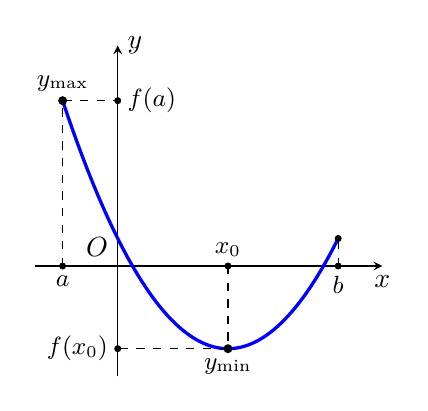
\begin{tikzpicture}[smooth,samples=300,scale=0.7,>=stealth]
	\draw[->] (-1.5,0)--(4.8,0) node[below]{$x$};
	\draw[->] (0,-2)--(0,4) node[right]{$y$};
	\draw (0,0) node[above left]{$O$};
	\draw[line width = 1.2pt,domain=-1:4,blue] plot(\x,{0.5*((\x)^2-4*(\x)+1)});
	\draw[fill=black] (-1,0) circle(1.5pt) (-1,3) circle(2pt) (0,3) circle(1.5pt) (0,-1.5) circle(1.5pt) (2,0) circle(1.5pt) (2,-1.5) circle(2pt) (4,0) circle(1.5pt) (4,0.5) circle(1.5pt);
	\draw[dashed] (-1,0)node[below]{\small$a$}--(-1,3)--(0,3)node[right]{\small$f(a)$} (2,0)node[above]{\small$x_0$}--(2,-1.5)--(0,-1.5)node[left]{\small$f(x_0)$}
	(4,0)node[below]{\small$b$}--(4,0.5);
	\node[above] at (-1,3) {\small $y_{\max}$};
	\node[below] at (2,-1.5) {\small $y_{\min}$};
\end{tikzpicture}}
\begin{note}
	\begin{listEX}[1]
		\item [\ding{172}] Khi yêu cầu tìm max min của hàm số mà không nói rõ xét trên tập nào, thì ta hiểu là tìm max min trên miền xác định của hàm số đó.
		\item [\ding{173}] Để tìm max min của hàm số $y=f(x)$ trên miền $\mathscr{D}$, ta thường lập bảng biến thiên của hàm số $y=f(x)$ trên $\mathscr{D}$. Từ bảng biến thiên, ta kết luận:
		\begin{itemize}
			\item [$\bullet$] Điểm ở vị trí cao nhất $\longrightarrow$ Kết luận max;
			\item [$\bullet$] Điểm ở vị trí thấp nhất $\longrightarrow$ Kết luận min.
		\end{itemize}
		\item [\ding{174}] Để tìm max min của hàm số $y=f(x)$ trên đoạn $[a;b]$ (\textit{$f(x)$ liên tục trên đoạn $[a ; b]$ và có đạo hàm trên $(a ; b)$ (có thể trừ một số hữu hạn các điểm) và $f^{\prime}(x)=0$ chỉ tại một số hữu hạn các điểm trong $(a ; b)$}), thì ta có thể giải như sau:
		\begin{itemize}
			\item [$\bullet$] Giải $f'(x)=0$ tìm các nghiệm $x_0 \in (a;b)$; 
			\item [$\bullet$] Tìm các điểm $x_i\in (a;b)$ mà tại đó đạo hàm không xác định (nếu có).
			\item [$\bullet$] Tính toán $f(a)$, $f(x_0)$, $f(x_i)$, $f(b)$ \quad ($\star$)
			\item [$\bullet$]  Gọi $M$, $n$ lần lượt là số lớn nhất và số nhỏ nhất của các kết quả tính toán ở bước ($\star$) thì
			$$M=\displaystyle\max_{[a;b]}f(x); \quad n=\displaystyle\min_{[a;b]}f(x)$$
		\end{itemize}
	\item [\ding{175}] Ta có thể dùng các bất đẳng thức có sẵn để đánh giá biểu thức cần tìm max, min. 
	% \begin{itemize}
	% 	\item [$\bullet$] Bất đẳng thức Cauchy cho hai số không âm $a$, $b$:
	% 	$$a+b \ge 2\sqrt{ab}$$
	% 	Dấu "=" xảy ra khi $a=b$.
	% 	\item [$\bullet$]  Bất đẳng thức Cauchy cho ba số không âm $a$, $b$, $c$:
	% 	$$a+b +c\ge 3\sqrt[3]{abc}$$
	% 	Dấu "=" xảy ra khi $a=b=c$.
	% 	\item [$\bullet$]  Bất đẳng thức Cauchy cho $n$ số không âm $a_1$, $a_2$,..., $a_n$:
	% 	$$a_1+a_2 +...+a_n \ge n\sqrt[n]{a_1a_2...a_n}$$
	% 	Dấu "=" xảy ra khi $a_1=a_2=...=a_n$.
	% \end{itemize}
	\end{listEX}
\end{note}
% \newpage
\subsection{PHÂN LOẠI VÀ PHƯƠNG PHÁP GIẢI TOÁN}
\begin{dang} {Bài toán tìm max, min của hàm số $y=f(x)$ trên miền $\mathscr{D}$}
	\begin{enumerate}[\iconMT]
		\item \indam{Phương pháp giải:} 
		\begin{listEX}[1]
			\item [\ding{172}] Tính $y'$. Giải phương trình $y'=0$ tìm các nghiệm $x_i \in \mathscr{D}$ và tìm các điểm $x_j \in \mathscr{D}$ mà tại đó $y'$ không xác định.
			\item [\ding{173}] Lập bảng biến thiên của hàm số trên $\mathscr{D}$.
			\item [\ding{174}] Từ bảng biến thiên, kết luận:
			\begin{itemize}
				\item [$\bullet$] Điểm ở vị trí cao nhất $\longrightarrow$ Kết luận max;
				\item [$\bullet$] Điểm ở vị trí thấp nhất $\longrightarrow$ Kết luận min.
			\end{itemize}
		\end{listEX}
		\item \indam{Lưu ý:} Nếu $\mathscr{D}$ là đoạn $\left[a;b\right]$ và hàm số $y=f(x)$ liên tục trên đoạn $\left[a;b\right]$ thì ta có thể làm như sau:
		\begin{listEX}[1]
			\item [\ding{172}] Giải $f'(x)=0$ tìm các nghiệm $x_0 \in (a;b)$;
			\item [\ding{173}] Tìm các điểm $x_i\in (a;b)$ mà tại đó đạo hàm không xác định (nếu có).
			\item [\ding{174}] Tính toán $f(a)$, $f(x_0)$, $f(x_i)$, $f(b)$ \quad ($\star$)
			\item [\ding{175}] Gọi $M$, $n$ lần lượt là số lớn nhất và số nhỏ nhất của các kết quả tính toán ở bước ($\star$) thì
			$$M=\displaystyle\max_{[a;b]}f(x); \quad n=\displaystyle\min_{[a;b]}f(x)$$
		\end{listEX}
		\begin{note}
			\begin{itemize}
				\item[\iconCH] Nếu hàm số $y=f(x)$ đồng biến trên đoạn $\left[a;b\right]$ thì $\min\limits_{[a;b]} f(x)=f(a)$ và $\max\limits_{[a;b]} f(x)=f(b)$.
				\item[\iconCH]  Nếu hàm số $y=f(x)$ nghịch biến trên đoạn $\left[a;b\right]$ thì $\min\limits_{[a;b]} f(x)=f(b)$ và $\max\limits_{[a;b]} f(x)=f(a)$.
			\end{itemize}
		\end{note}
	\end{enumerate}
\end{dang}

\boxmini{BÀI TẬP TỰ LUẬN}
\begin{vd}
	Tìm giá trị lớn nhất và nhỏ nhất (nếu có) của hàm số sau trên đoạn đã chỉ ra.
	\begin{tasks}(2)
		\task $f(x)=-x^3+3x^2+10$ trên đoạn $[-3;1]$.
		\task $f(x)=\dfrac{x^3}{3}-2x^2+3x+1$ trên đoạn $[-3;2]$.
		\task $f(x) = - 2x^4 + 4x^2 + 3$ trên đoạn $\left[0;2\right]$
		\task $f(x)=\dfrac{2x+3}{x+1}$ trên đoạn $[0;4]$.
		\task $f(x)=x+\dfrac{4}{x}$ trên khoảng $(0;+\infty)$;
		\task $f(x)=3x+\dfrac{4}{x^2}$ trên $(0;+\infty)$.
		\task $f(x)=\dfrac{2x^2+4x+5}{x^2+1}$ trên $\mathbb{R}$.
		\task $f(x)=\sqrt{-x^2+2x}$ trên miền xác định.
	\end{tasks}
\loigiai{
\begin{enumerate}[a)]
	\item Hàm số liên tục trên $[-3;1]$. Ta có $f'(x)=-3x^2+6x$; $f'(x)=0 \,\Leftrightarrow \hoac{&x=0 \in [-3;1]\\&x=2 \notin [-3;1]}$.\\
	Ta có $f(-3)=64$, $f(0)=10$, $f(1)=12$. Suy ra, $\max\limits_{[-3;1]} f(x)=f(-3)=64$; $\min\limits_{[-3;1]} f(x)=f(0)=10$.
	
	\item Hàm số liên tục trên $[-3;2]$
	Ta có $f^{\prime}(x)=x^2-4x+3$; $f^{\prime}(x)=0\Leftrightarrow \heva{&x=1\\x=3\notin[-3;2]}$.\\
	$f(1)=\dfrac{7}{3}$, $f(3)=-35$, $f(2)=\dfrac{5}{3}$.\\
	Vậy 
	$\max\limits_{[-3;2]}f(x)=\dfrac{7}{3}$ và
	$\min\limits_{[-3;2]}f(x)=-35$.	
	\item Ta có $f'(x)=- 8x^3 + 8x =- 8x(x^2 - 1) =- 8x(x - 1)(x + 1)$.\\
	Xét $f(0) = 3$, $f(1) = 5$ và $f(2) =- 13$.\\
	Vậy 
	$\max\limits_{[0;2]}f(x)=5$ và
	$\min\limits_{[0;2]}f(x)=-13$.	
	\item Hàm số đã cho liên tục trên đoạn $[0;4]$.\\
	Ta có $y'=-\dfrac{1}{(x+1)^2} < 0$, $\forall x \in [0;4]$. Suy ra hàm số đã cho nghịch biến trên đoạn $[0;4]$.\\
	Vậy $\max\limits_{[0;4]} y = y(0) = 3$ và $\min\limits_{[0;4]} y = y(4) = \dfrac{11}{5}$.
	
	\item Xét hàm số $f(x)=x+\dfrac{4}{x}$ trên khoảng $(0;+\infty)$.\\
	Đạo hàm $f'(x)=1-\dfrac{4}{x^2}=\dfrac{x^2-4}{x^2}$.\\
	Cho $f'(x)=0 \Leftrightarrow x^2-4=0 \Leftrightarrow \hoac{&x=2\in(0;+\infty)\\&x=-2\notin(0;+\infty).}$\\
	Bảng biến thiên
	\begin{center}
		
\begin{tikzpicture}[font=\footnotesize,thick,>=stealth]
			\tikzset{double style/.append style={double distance=1.75pt}}
			\tkzTabInit[nocadre=false,lgt=1.2,espcl=2.5,deltacl=0.6,lw=.5pt,color,colorL=green!50,colorV=green!50]
			{$x$ /0.6,$f'(x)$ /0.6,$f(x)$ /2}
			{$-\infty$,$-2$,$0$,$2$,$+\infty$}
			\tkzTabLine{,+,$0$,-,d,-,$0$,+,}
			\tkzTabVar{-/$-\infty$,+/$-4$,-D+/$-\infty$/$+\infty$,-/$4$,+/$+\infty$}
			%\draw[pattern={Lines[angle=60,distance=1.25mm]},pattern color=blue,thin] (N11)--(N31)--(N33)--(N13);
		\end{tikzpicture}
	\end{center}
	Căn cứ vào bảng biến thiên, ta có $\min\limits_{(0;+\infty)}f(x)=4$.
	
	\item Áp dụng bất đẳng thức Cauchy cho $3$ số dương, ta có
	$$y=\dfrac{3x}{2}+\dfrac{3x}{2}+\dfrac{4}{x^2} \geq 3\sqrt[3]{\dfrac{3x}{2}\cdot \dfrac{3x}{2}\cdot \dfrac{4}{x^2}}=3\sqrt[3]{9}.$$
	Đẳng thức xảy ra khi $\dfrac{3x}{2}=\dfrac{4}{x^2} \Leftrightarrow x=\dfrac{2}{\sqrt[3]{2}}=2\sqrt[3]{2}$.
	
	\item Tập xác định $\mathscr{D}= \mathbb{R}$.\\
	Ta có $y'= \dfrac{-4x^2-6x+4}{(x^2+1)^2}$, \; $y'=0 \Leftrightarrow -4x^2-6x+4=0\Leftrightarrow \hoac{&x=-2\\&x=\dfrac{1}{2}.}$
	\begin{center}
		
\begin{tikzpicture}\tkzTabInit[nocadre=false,lgt=1.2,espcl=2.5,deltacl=0.6]
			{$x$ /1, $y'$ /0.6, $y$ /2.5}
			{$-\infty$,$-2$,$\dfrac{1}{2}$,$+\infty$}
			\tkzTabLine{,-,$0$,+,$0$,-,}
			\tkzTabVar{+/$2$,-/$1$,+/$6$,-/$2$}
		\end{tikzpicture}
	\end{center}
	Suy ra $M=6$ và $m=1$.
	
	\item Hàm số $f(x)=\sqrt{-x^2+2x}$ liên tục trên $[0;2]$.\\
	$f'(x)=\dfrac{1-x}{\sqrt{-x^2+2x}}$, $f'(x)=0 \Leftrightarrow x=1$.\\
	Ta có $f(0)=0$, $f(2)=0$, $f(1)=1$.\\
	Vậy $\displaystyle\max_{x\in [0;2]}f(x)=1$ và $\displaystyle\min_{x\in [0;2]}f(x)=0$.
\end{enumerate}}
\end{vd}
\dongcham{54}
\begin{vd}
	Tìm giá trị lớn nhất và nhỏ nhất của hàm số sau trên miền đã chỉ ra.
	\begin{tasks}(2)
		\task $y=x-\sin 2x$ trên đoạn $\left[-\dfrac{\pi}{2};\pi\right]$
		\task $y = \mathrm{e}^{x^3 - 3x + 3}$ trên đoạn $[0; 2]$
		\task $y=\mathrm{e}^{x}(x^{2}-3)$ trên đoạn $[-2;2]$
		\task $y=\dfrac{\ln^2x}{x}$ trên đoạn $\left[1;\mathrm{e}^5\right]$
	\end{tasks}
	\loigiai{
		\begin{enumerate}[a)]
			\item Ta có
			\begin{itemize}
				\item $y'=1-2\cos 2x$.
				\item $\heva{&x\in \left(-\dfrac{\pi}{2};\pi\right)\\& y'=0}\Leftrightarrow \heva{&x\in \left(-\dfrac{\pi}{2};\pi\right)\\&\cos 2x=\dfrac{1}{2}}\Leftrightarrow \heva{&x\in \left(-\dfrac{\pi}{2};\pi\right)\\&x=\pm \dfrac{\pi}{6}+k\pi} \Leftrightarrow \hoac {&x=\pm\dfrac{\pi}{6}\\& x=\dfrac{5\pi}{6}.}$
				\item $f\left(-\dfrac{\pi}{2}\right)=-\dfrac{\pi}{2}$,  $f(\pi)=\pi$,
				$f\left(-\dfrac{\pi}{6}\right)=-\dfrac{\pi}{6}+\dfrac{\sqrt{3}}{2}$,  $f\left(\dfrac{\pi}{6}\right)=\dfrac{\pi}{6}-\dfrac{\sqrt{3}}{2}$,  $f\left(\dfrac{5\pi}{2}\right)=\dfrac{5\pi}{6}+\dfrac{\sqrt{3}}{2}$.
			\end{itemize}
			Vậy giá trị lớn nhất và giá trị nhỏ nhất của hàm số $y=x-\sin 2x$ trên đoạn $\left[-\dfrac{\pi}{2};\pi\right]$ lần lượt là $\dfrac{5\pi+3\sqrt{3}}{6}$ và $-\dfrac{\pi}{2}$.
			\item Ta có $y' = (3x^2 - 3)\cdot \mathrm{e}^{x^3 - 3x + 3}$.\\
			$y' = 0 \Leftrightarrow 3x^2 - 3 = 0 \Leftrightarrow x = 1$ do $x \in [0;2]$.\\
			Khi đó $y(0) = \mathrm{e}^3$; $y(2) = \mathrm{e}^5$; $y(1) = \mathrm{e}$.
			Vậy $ \max \limits_{[0; 2]} y = \mathrm{e}^5 $ khi $x = 2$.
			\item Ta có $y'=\mathrm{e}^x(x^2+2x-3)=0\Leftrightarrow \hoac{&x=-3\\ &x=1}$.
			Xét các giá trị: $f(-2)=\mathrm{e}^{-2}$; $f(1)=-2\mathrm{e}$; $f(2)=\mathrm{e}^2$, từ đó suy ra $y_{\min}=-2\mathrm{e}$.
			\item $y'=\dfrac{2\ln x-\ln^2x}{x^2}$, $y'=0\Leftrightarrow \hoac{
				& \ln x=0 \\
				& \ln x=2 \\} \Leftrightarrow \hoac{
				& x=1 \\
				& x=\mathrm{e}^2. \\}$\\
			Tính $y(1)=0$, $y(\mathrm{e}^2)=\dfrac{4}{\mathrm{e}^2}\approx 0{,}54$, $y(\mathrm{e}^5)=\dfrac{9}{\mathrm{e}^5}\approx 0{,}16$.\\
			Vậy $\max\limits_{x \in \left[1;\mathrm{e}^5\right]}y=\dfrac{4}{\mathrm{e}^2}$
	\end{enumerate}}
\end{vd}
\dongcham{40}
\begin{vd}
	Tìm giá trị lớn nhất và nhỏ nhất (nếu có) của hàm số sau trên miền đã chỉ ra.
	\begin{tasks}(2)
		\task $f(x)=\dfrac{5\sin x+1}{\sin x+2}$ trên đoạn $\left[0;\dfrac{\pi}{6}\right]$.
		\task $ y=\cos^3x +2\sin^2x+\cos x$ trên miền xác định.
	\end{tasks}
	\loigiai{
		\begin{enumerate}[a)]
			\item Đặt $t=\sin x,\; x\in \left[0;\dfrac{\pi}{6}\right]\Rightarrow t \in \left[0;\dfrac{1}{2}\right]$.\\
			Ta được hàm số $y=g(t)=\dfrac{5t+1}{t+2}$.\\
			$g'(t)=\dfrac{9}{(t+2)^2}>0,\forall t \in \left[0;\dfrac{1}{2}\right]$.\\
			Vì $g(0)=\dfrac{1}{2}$, $g\left(\dfrac{1}{2}\right)=\dfrac{7}{5}$ nên $\min\limits_{\left[0;\tfrac{1}{2}\right]}g(t)=g(0)=\dfrac{1}{2}.$\\
			Vậy $\min\limits_{\left[0;\tfrac{\pi}{6}\right]}f(x)=\min\limits_{\left[0;\tfrac{1}{2}\right]}g(t)=\dfrac{1}{2}$
			\item Ta có $ y=\cos^3x +2\sin^2x+\cos x =\cos^3x +2(1-\cos^2x)+\cos x =\cos^3x-2\cos^2x+\cos x+2$.\\
			Đặt $ t=\cos x,\, t\in [-1;1] $. Ta được $ f(t)=t^3-2t^2 +t+2$.\\
			Ta có $ f'(t)=3t^2-4t+1;\,y'=0\Leftrightarrow \hoac{&t=1\in[-1;1]\\&t=\dfrac{1}{3}\in[-1;1].} $\\
			Mà $f\left(-1\right)=-2$, $ f\left(\dfrac{1}{3}\right)=\dfrac{58}{27} $, $f(1)=2$ nên $\max\limits_{x\in \mathbb{R}}y=\max\limits_{\left[-1;1\right]}f(t)=\dfrac{58}{27}$
			\item
			\item
	\end{enumerate}}
\end{vd}
\dongcham{43}
\boxmini{BÀI TẬP TRẮC NGHIỆM}
\ind{PHẦN I.} \inden{Câu trắc nghiệm nhiều phương án lựa chọn. Mỗi câu hỏi học sinh chỉ chọn một phương án.}\\
\setcounter{ex}{0}
\Opensolutionfile{ans}[ans/2D1-B2-d1-1]

\begin{ex}
	\immini
	{Hàm số $y=f(x)$ liên tục trên đoạn $[-1;3]$ và có bảng biến thiên như sau.\\
		Gọi $M$ là giá trị lớn nhất của hàm số $y=f(x)$ trên đoạn $[-1;3]$. Khẳng định nào sau đây là khẳng định đúng?
		\choice
		{\True $M=f(0)$}
		{$M=f(-1)$}
		{$M=f(3)$}
		{$M=f(2)$}
	}
	{
\begin{tikzpicture}
			\tkzTabInit[nocadre=True,lgt=1.2,espcl=2]
			{$x$ /0.7,$y'$ /0.7,$y$ /2.1}
			{$-1$,$0$,$2$,$3$}
			\tkzTabLine{,+,$0$,-,$0$,+,}
			\tkzTabVar{-/$0$, +/$5$,-/$1$,+/$4$}
	\end{tikzpicture}}
	\loigiai
	{Dựa vào bảng biến thiên ta có $M=f(0)=5$.}
\end{ex} \dongcham{1}

\begin{ex}
	\immini{Cho hàm số $f(x)$ liên tục trên đoạn $[-1;5]$ và có đồ thị như hình vẽ bên. Gọi $M$ và $m$ lần lượt là giá trị lớn nhất và nhỏ nhất của hàm số đã cho trên $[-1;5]$. Giá trị của $M+m$ bằng
		\choice
		{$5$}
		{$6$}
		{$3$}
		{\True $1$}
	}{
		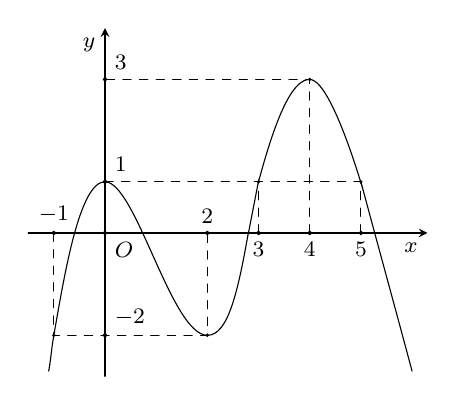
\begin{tikzpicture}[scale=0.65, font=\footnotesize, line join=round, line cap=round, >=stealth]
			%%Nhập giới hạn đồ thị và hàm số cần vẽ
			\def \xmin{-1.5}
			\def \xmax{6.3}
			\def \ymin{-2.8}
			\def \ymax{4}
			%%Tự động
			\draw[->] (\xmin,0)--(\xmax,0) node[below left] {$x$};
			\draw[->] (0,\ymin)--(0,\ymax) node[below left] {$y$};
			\draw[fill=black] (0,0) circle(1pt) node [below right] {$O$};
			%%Vẽ các điểm trên 2 hệ trục
			\foreach \x in {3,4,5}
			\draw[fill=black] (\x,0) circle(1pt) node [below] {$\x$};
			\foreach \x in {-1,2}
			\draw[fill=black] (\x,0) circle(1pt) node [above] {$\x$};
			\foreach \y in {-2,1,3}
			\draw[fill=black] (0,\y) circle(1pt) node [above right] {$\y$};
			\draw[dashed](-1,0)--(-1,-2)--(0,-2)--(2,-2)--(2,0) (5,0)--(5,1)--(0,1) (3,0)--(3,1) (4,0)--(4,3)--(0,3);
			%%Tự động
			\draw
			(-1.1,-2.7) to[out=80, in=-100] (-1,-2)
			..controls +(80:1.2) and +(180:.5)..(0,1)
			..controls +(0:.6) and +(180:0.7)..(2,-2)
			..controls +(0:0.4) and +(-100:1.2)..(2.8,0)
			to[in=80, out=-100] (3,1)
			..controls +(75:1.5) and +(180:0.3)..(4,3)
			..controls +(0:0.5) and +(-75:1)..(5,1)
			to[in=105, out=-75] (6,-2.7);
			\fill[black]
			(-1,-2) circle(1pt)
			(2,-2) circle(1pt)
			(3,1) circle(1pt)
			(4,3) circle(1pt)
			(5,1) circle(1pt)
			;
		\end{tikzpicture}
	}
	\loigiai{
		Dựa vào đồ thị, suy ra $m=\min\limits_{[-1;5]} f(x)=f(-1)=-2$, $M=\max\limits_{[-1;5]} f(x)=f(4)=3$.\\
		Do đó $M+m=3-2=1$.
	}
\end{ex} \dongcham{1}

\begin{ex}
	\immini{Cho hàm số $y=f(x)$ có đồ thị là đường cong ở hình bên. Tìm giá trị nhỏ nhất $m$ của hàm số $y=f(x)$ trên đoạn $[-1;1] $.
		\haicot
		{$m=2 $}
		{\True $m=-2 $}
		{$m=1 $}
		{$m=-1 $}}{\vspace{-0.5cm}
		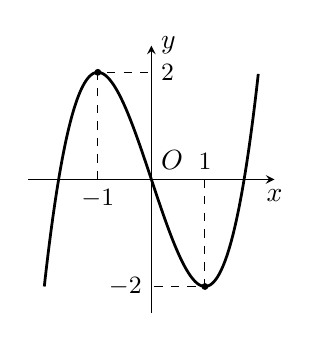
\begin{tikzpicture}[smooth,samples=300,scale=0.68,>=stealth]
			\draw[->] (-2.3,0)--(2.3,0) node[below]{$x$};
			\draw[->] (0,-2.5)--(0,2.5) node[right]{$y$};
			\draw (0,0) node[above right]{$O$};
			\draw[line width = 1pt,domain=-2:2] plot(\x,{(\x)^(3)-3*(\x)});
			\draw[fill=black] (-1,2) circle(1.5pt) (1,-2) circle(1.5pt);
			\draw[dashed] (-1,0)node[below]{\small$-1$}--(-1,2)--(0,2)node[right]{\small$2$} (1,0)node[above]{\small$1$}--(1,-2)--(0,-2)node[left]{\small$-2$};
	\end{tikzpicture}}
	\loigiai{
		Dựa vào đồ thị ta có giá trị nhỏ nhất của hàm số trên đoạn $[-1;1] $ bằng $-2$.	
		
	}
	
\end{ex} \dongcham{1}

\begin{ex}
	Cho hàm số $y=f(x)$ có bảng biến thiên trên đoạn $[-2;3]$ như hình bên dưới.
	\begin{center}
		
\begin{tikzpicture}[>=stealth,scale=1]
			\tkzTabInit[nocadre=false,lgt=1.2,espcl=2,deltacl=0.6]
			{$x$/0.6,$f’(x)$/0.6,$f(x)$/2}
			{$-\infty$,$-2$,$-1$,$1$,$3$,$+\infty$}
			\tkzTabLine{,h,,+,z,-,d,+,,h}
			\tkzTabVar{+H/,-/$0$,+/$1$,-/$-2$,+H/$5$}
		\end{tikzpicture}
	\end{center}
	Gọi $M$ và $m$ lần lượt là giá trị lớn nhất và giá trị nhỏ nhất của hàm số đã cho trên đoạn $[-1;3]$. Giá trị của biểu thức $M-m$ là
	\choice
	{$5$}
	{\True $7$}
	{$-1$}
	{$3$}
	\loigiai{
		Dựa vào bảng biến thiên ta thấy giá trị lớn nhất của hàm số là $M=5$ và giá trị nhỏ nhất của hàm số là $m=-2$ nên $M-m=7$.}
\end{ex}
% \newpage
\begin{ex}
	Giá trị lớn nhất và nhỏ nhất của hàm số $y=x^3-12x+1$ trên đoạn $[-2;3]$ lần lượt là
	\choice
	{\True $17$, $-15$}
	{$10$, $-26$}
	{$-15$, $17$}
	{$6$, $-26$}
	\loigiai{
		Ta có $y'=3x^2-12$, do đó $y'=0\Leftrightarrow 3x^2-12=0\Leftrightarrow x=\pm 2\in [-2;3]$.\\
		Mặt khác $f(-2)=17$, $f(2)=-15$, $f(3)=-8$.\\
		Vậy giá trị lớn nhất và nhỏ nhất cần tìm lần lượt là $17$, $-15$.
	}
\end{ex} \dongcham{12}

\begin{ex}
	Gọi $ M, m $ lần lượt là giá trị lớn nhất và giá trị nhỏ nhất của hàm số $ y = x^3 + 3x^2 - 9x + 1 $ trên $ [-4;4] $. Tính tổng $ M + m. $
	\choice 
	{$ 12 $}
	{$ 98 $}
	{$ 17 $}
	{\True $ 73 $}
	\loigiai
	{
		Ta có $ y' = 3x^2 + 6x - 9 = 0 \Leftrightarrow \hoac{&x = 1\\ &x = -3.} $\\
		Khi đó: $ y(-4) = 21 $,\, $ y(-3) = 28, $
		\, $ y(1) = -4, $
		\, $ y(4) = 77. $\\
		Do đó $ M + m = 77 + (-4) = 73. $
	}
\end{ex} \dongcham{12}

\begin{ex}
	Giá trị lớn nhất của hàm số $f(x)=-x^4+12x^2+1$ trên đoạn $\left[ -1;2\right] $ bằng
	\choice
	{\True $33$}
	{$37$}
	{$12$}
	{$1$}
	\loigiai{
		Hàm số $f(x)=-x^4+12x^2+1$ liên tục trên đoạn $\left[ -1;2\right] $.\\
		Ta có $f'(x)=-4x^3+24x=-4x(x^2-6)$.\\
		$f'(x)=0 \Leftrightarrow \hoac{& x=-\sqrt{6} \not \in \left[ -1;2\right] \\ &x=0 \in \left[ -1;2\right] \\&x=\sqrt{6} \not \in \left[ -1;2\right]. }$\\
		Ta có $f(-1)=12; f(0)=1; f(2)=33$.\\
		Vậy $\max\limits_{\left[ -1;2\right] } f(x)=33$.
	}
\end{ex} \dongcham{12}
\begin{ex}
	Giá trị lớn nhất của hàm số $y=x^4-3x^2+2$ trên đoạn $\left[ 0;3\right] $ bằng
	\choice
	{ $ 57 $}
	{\True $ 56 $}
	{$ 54$}
	{$ 55 $}
	\loigiai{
		Hàm số $y$ liên tục trên đoạn $\left[ 0;3\right] $ và có đạo hàm $y'=4x^3-6x$.\\
		Ta có $y'=0 \Leftrightarrow 4x^3-6x=0 \Leftrightarrow \hoac{& x=0 \in \left[ 0;3\right]  \\&x=\sqrt{\dfrac{3}{2}} \in \left[ 0;3\right]\\ & x=- \sqrt{\dfrac{3}{2}}\notin \left[ 0;3\right].}$\\
		Ta có $y(0)=2$, $y(3)=56$, $y\left(\sqrt{\dfrac{3}{2}}\right) =-\dfrac{1}{4} $.\\
		Do đó giá trị lớn nhất của hàm số $y=x^4-3x^2+2$ trên đoạn $\left[ 0;3\right] $ bằng $56$.
	}
\end{ex} \dongcham{7}

\begin{ex}%[2D1Y3-1]
	Giá trị nhỏ nhất của hàm số $y=\dfrac{x-1}{x+1}$ trên đoạn $[0;3]$ là
	\choice
	{$\min\limits_{[0;3]}y=\dfrac{1}{2}$}
	{$\min\limits_{[0;3]}y=-3$}
	{$\min\limits_{[0;3]}y=1$}
	{\True $\min\limits_{[0;3]}y=-1$}	
	\loigiai{
		Trên đoạn $[0;3]$ hàm số luôn xác định.\\
		Ta có $y'=\dfrac{2}{(x+1)^2}>0$, $\forall x \in [0;3]$ nên hàm số đã cho đồng biến trên đoạn $[0;3]$.\\
		Do đó $\min\limits_{[0;3]}y=y(0)=-1$.
	}	
\end{ex} \dongcham{7}

\begin{ex}%
	Giá trị nhỏ nhất của hàm số $y=\dfrac{2x+3}{x+1}$ trên đoạn $[0;4]$ là
	\choice
	{$2$}
	{$\dfrac{7}{5}$}
	{$3$}
	{\True $\dfrac{11}{5}$}
	\loigiai
	{
		Ta có $y'=\dfrac{-1}{(x+1)^2}<0$ nên $\min\limits_{[0;4]} y=y(4)=\dfrac{11}{5}$.
	}
\end{ex} \dongcham{7}

\begin{ex}%[2D1B3]
	Giá trị lớn nhất của hàm số $y=\dfrac{x^2-3x+3}{x-1}$ trên đoạn $\left[-2;\dfrac{1}{2}\right]$ bằng
	\choice
	{$4$}
	{\True $-3$}
	{$-\dfrac{7}{2}$}
	{$-\dfrac{13}{3}$}
	\loigiai{
		Ta có $y'=\dfrac{x^2-2x}{(x-1)^2}$. Xét $y'=0\Leftrightarrow  x^2-2x=0\Leftrightarrow \hoac{&x=0\in \left[-2;\dfrac{1}{2}\right]\\&x=2\notin\left[-2;\dfrac{1}{2}\right]}$.\\
		Ta có $y(0)=-3$, $y(-2)=\dfrac{-13}{3}$, $y\left(\dfrac{1}{2}\right)=\dfrac{-7}{2}$.\\
		Suy ra $\underset{x\in \left[-2;\dfrac{1}{2}\right]}{\max y}=-3$
	}
\end{ex} \dongcham{10}

\begin{ex}
	Giá trị lớn nhất của hàm số $y=\sqrt{4-x^2}$ là
	\choice
	{$M=-2$}
	{\True $M=2$ }
	{$M=4$}
	{$M=0$}
	\loigiai
	{
		Tập xác định: $\mathscr{D}=\left[-2;2\right]$.\\
		Đạo hàm $y'=\dfrac{-x}{\sqrt{4-x^{2}}}$; $y'=0 \Leftrightarrow x=0 \in \left[-2;2\right]$.\\
		Ta có $y(2)=y(-2)=0$; $y(0)=2$.\\
		Vậy giá trị lớn nhất của hàm số đã cho bằng $2$.
	}
\end{ex} \dongcham{8}

\begin{ex}%[2D1B3-1]
	Tìm giá trị lớn nhất $M$ của hàm số $y=\sqrt{7+6x-x^2}$.
	\choice
	{\True $M=4$}
	{$M=\sqrt{7}$}
	{$M=7$}
	{$M=3$}
	\loigiai{
		Tập xác định $\mathscr{D}=[-1;7]$.\\
		$y'=\dfrac{-x+3}{\sqrt{7+6x-x^2}}$.\\
		Cho $y'=0\Leftrightarrow x= 3\in \mathscr{D}$.\\
		Có $y(3)=4, y(-1)=0, y(7)=0$. Vậy $M=4$.	
	}
\end{ex} \dongcham{8}

\begin{ex}%[Nguyễn Quang Hiệp - Phát triển đề minh họa 2021]%[2D2B4-4]%
	Tính giá trị lớn nhất của hàm số $y=x-\ln x$ trên $\left[\dfrac{1}{2};\mathrm{e}\right]$.\\
	\choice
	{$\max\limits_{x \in \left[\frac{1}{2};\mathrm{e}\right]}y=1$}
	{\True $\max\limits_{x \in \left[\frac{1}{2};\mathrm{e}\right]}y=\mathrm{e}-1$}
	{$\max\limits_{x \in \left[\frac{1}{2};\mathrm{e}\right]}y=\mathrm{e}$}
	{$\max\limits_{x \in \left[\frac{1}{2};\mathrm{e}\right]}y=\dfrac{1}{2}+\ln 2$}
	\loigiai{
		Hàm số $y=x-\ln x$liên tục trên đoạn $\left[\dfrac{1}{2};\mathrm{e}\right]$.\\
		Ta có $y'=1-\dfrac{1}{x}\Rightarrow y'=0\Leftrightarrow x=1\in \left[\dfrac{1}{2};\mathrm{e}\right]$.\\
		Do $y\left(\dfrac{1}{2}\right)=\dfrac{1}{2}+\ln 2$; $y(\mathrm{e})=\mathrm{e}-1$; $y(1)=1$ nên $\max\limits_{x \in \left[\frac{1}{2};\mathrm{e}\right]}y=\mathrm{e}-1$.}
\end{ex} \dongcham{8}

\begin{ex}
	Gọi $M, N$ lần lượt là giá trị lớn nhất và nhỏ nhất của hàm số $y = x^2 - 4\ln (1 - x)$ trên đoạn $[-2;0]$. Tính $M - N$.
	\choice
	{$M - N = 4\ln 2$}
	{$M - N = -1$}
	{\True $M - N = 4\ln 2 -1$}
	{$M - N = 4\ln 3 -4$}
	\loigiai{
		Tập xác định: $\mathscr{D} = (-\infty;1)$.\\
		Ta có $y' = 2x + \dfrac{4}{1 - x} = \dfrac{-2x^2 + 2x + 4}{1 - x}$.\\
		Khi đó $y' = 0 \Leftrightarrow -2x^2 + 2x + 4 = 0 \Leftrightarrow \hoac{&x = -1 \quad \mbox{(nhận)} \\&x = 2 \quad \mbox{(loại)}. }$\\
		Khi đó $\heva{& y(-2) = 4 - 4\ln 3 \approx -0{,}4 \\& y(-1) = 1 - 4\ln 2  \approx -1{,}7\\& y(0) = 0.} \Rightarrow M = 0, N = 1 -4\ln 2$\\
		Vậy $M - N = 4\ln 2 -1$.
	}
\end{ex} \dongcham{8}

\begin{ex}
	Cho hàm số $f(x)$ nghịch biến trên $\mathbb{R}$. Giá trị nhỏ nhất của hàm số $g(x)=\mathrm{e}^{3x^2-2x^3}-f(x)$ trên đoạn $[0;1]$ bằng
	\choice
	{$\mathrm{e}-f(1)$}
	{$f(1)$}
	{$f(0)$}
	{\True $1-f(0)$}
	\loigiai{
		Ta có $g'(x)=(6x-6x^2)\mathrm{e}^{3x^2-2x^3}-f'(x)$.\\
		Trên đoạn $[0;1]$ thì $6x-6x^2\ge 0$, $f'(x)\le 0$ nên $g'(x)\ge 0$, suy ra hàm số $g(x)$ đồng biến, suy ra giá trị nhỏ nhất là $g(0)=1-f(0)$.
	}
\end{ex} \dongcham{8}

\begin{ex}
	\immini{Cho hàm số $y=f(x)$ xác định và liên tục trên đoạn $\left[0;\dfrac{7}{2}\right]$, có
		đồ thị của hàm số $y=f'(x)$ như hình vẽ. Hỏi hàm số $y=f(x)$ đạt giá trị nhỏ nhất trên đoạn $\left[0;\dfrac{7}{2}\right]$ tại điểm $x_0$ nào dưới đây?
		\choice
		{\True $x_0=3$}
		{$x_0=2$}
		{$x_0=1$}
		{$x_0=0$}
	}
	{\begin{tikzpicture}[scale=1,font=\footnotesize, line join=round,line cap=round,>=stealth]
			\draw [->] (-1,0)--(0,0)
			node[below left]{$O$}--(4.5,0)node[below]{$x$}; % Hệ trục tọa độ
			\draw[->] (0,-1.5) --(0,2) node[left]{$y$};
			\draw[dashed](3.5,0)node[below]{$\tfrac{7}{2}$}--(3.5,25/16);
			\draw(1,0)node[above]{$1$}(3,0)node[above left]{$3$};
			\draw [domain=0:3.5,samples=100] plot (\x, {(\x-1)^2*(\x-3)/2});
	\end{tikzpicture}}
	\loigiai{
		Từ đồ thị hàm số ta có $f'(x)=0 \Leftrightarrow \hoac{&x=1\\&x=3.}$\\
		Bảng biến thiên của hàm số $y=f(x)$ trên đoạn $\left[0;\dfrac{7}{2}\right]$
		\begin{center}
			
\begin{tikzpicture}
				\tkzTabInit[nocadre=false,lgt=1.2,espcl=2.5,deltacl=0.7]{$x$ / 1.1 , $f’(x)$ /0.7, $f(x)$ / 2}
				{$0$,$1$, $3$ , $\dfrac{7}{2}$}%
				\tkzTabLine{,-,0,-,0,+,}%
				\tkzTabVar{+ /$f(0)$,R/,-/$f(3)$,+ / $f\left(\dfrac{7}{2}\right)$}%
				\tkzTabIma{1}{3}{2}{$f(0)$}
			\end{tikzpicture}
		\end{center}
		Từ bảng biến thiên ta có hàm số $y=f(x)$ đạt giá trị nhỏ nhất trên đoạn $\left[0;\dfrac{7}{2}\right]$ tại điểm $x_0=3.$
	}
\end{ex} \dongcham{10}

\begin{ex}%[2D1K3-1]
	\immini{Cho hàm số $y=f(x)$, biết hàm số $y=f'(x)$ có đồ thị như hình vẽ dưới đây. Hàm số $y=f(x)$ đạt giá trị nhỏ nhất trên đoạn $\left[\dfrac{1}{2};\dfrac{3}{2} \right]$ tại điểm nào sau đây?
		\choicew{0,25 \textwidth}
		\choice
		{$x=\dfrac{3}{2}$}
		{$x=\dfrac{1}{2}$}
		{\True $x=1$}
		{$x=0$}}{\vspace{-0.5cm}\begin{tikzpicture}[>=stealth,scale=1.5]
			\draw[->] (-0.5,0)--(2.5,0) node[below]{\footnotesize $x$};
			\draw[->] (0,-0.5)--(0,1.5) node[right]{\footnotesize $y$};
			\draw (0,0) node[below left]{\footnotesize $O$};
			\draw[line width = 1pt,smooth,domain=-0.4:1.7] plot({\x},{(\x)^2-\x});
			\draw[fill=black] (1.5,0.75) circle(1pt);
			\draw [dashed] (1.5,0)
			node[below]{\footnotesize$\dfrac{3}{2}$}--(1.5,0.75)--(0,0.75)(1,0)node[below]{$1$};
	\end{tikzpicture}}
	\loigiai{
		Dựa vào đồ thị hàm số $y=f'(x)$. Ta có bảng biến thiên
		\begin{center}
\begin{tikzpicture}
				\tkzTabInit[nocadre=false,lgt=1,espcl=2.1]
				{$x$ /1,$y'$ /0.6,$y$ /2}
				{$\dfrac{1}{2}$,$1$,$\dfrac{3}{2}$}
				\tkzTabLine{,-,$0$,+,$0$,}
				\tkzTabVar{+/, -/,+/}
			\end{tikzpicture}
		\end{center}
		Suy ra hàm số đạt giá trị nhỏ nhất trên $\left[\dfrac{1}{2};\dfrac{3}{2} \right]$ tại $x=1$.}
\end{ex} \dongcham{10}

\begin{ex}
	\immini{ Cho hàm số $f(x)$ có đồ thị của hàm số $y=f'(x)$ như hình vẽ. Biết $f(0)+f(1)-2f(2)=f(4)-f(3)$. Giá trị nhỏ nhất $m$, giá trị lớn nhất $M$ của hàm số $f(x)$ trên đoạn $[0;4]$ là
		\choice
		{$m=f(4)$, $M=f(1)$}
		{\True $m=f(4)$, $M=f(2)$}
		{$m=f(1)$, $M=f(2)$}
		{$m=f(0)$, $M=f(2)$}
	}{
		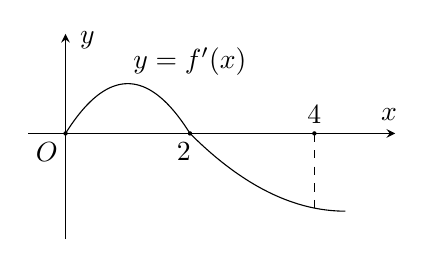
\begin{tikzpicture}[scale=0.79, >=stealth]
			\draw[->] (-0.6,0.) -- (5.3,0.);
			\draw[->] (0.,-1.7) -- (0.,1.6);
			\draw[dashed] (4,0) -- (4,-1.2);
			\clip(-0.6,-1.7) rectangle (5.3,1.7);
			\draw[smooth,samples=100,domain=0:2] plot(\x,{-0.8*((\x)^2-2*(\x))});
			\draw[smooth,samples=100,domain=2:4.5] plot(\x,{0.2*(((\x)-2)*((\x)-7)});
			\draw (-0.3,-0.3) node {$O$} (5.2,0.3) node {$x$} (0.35,1.5) node {$y$} (1.9,-0.3) node {$2$} (4.0,0.3) node {$4$} (2.0,1.15) node {$y=f'(x)$};
			\fill (0,0) circle(1pt) (2,0) circle(1pt) (4,0) circle(1pt); 
		\end{tikzpicture}
	}
	\loigiai{
		Từ đồ thị hàm số $y=f'(x)$ ta suy ra $f'(x)=0 \Leftrightarrow \hoac{&x=0\\&x=2.}$\\
		Ta có bảng biến thiên: 
		\begin{center}
\begin{tikzpicture}[>=stealth,scale=1]
				\tkzTabInit[lgt=1.2,espcl=2.5]
				{$x$/1,$f'(x)$/1,$f(x)$/2.5}
				{$0$,$2$,$4$}
				\tkzTabLine{$0$,+,$0$,- }
				\tkzTabVar{-/$f(0)$,+/$f(2)$,-/$f(4)$}
		\end{tikzpicture}\end{center}
		Từ bảng biến thiên ta thấy $M=f(2)$.\\
		Mặt khác, từ bảng biến thiên ta có $\heva{&f(1)<f(2)\\&f(3)<f(2)}\Rightarrow f(1)+f(3)<2f(2)$.\\
		Do đó $f(4)=f(0)+f(1)+f(3)-2f(2)<f(0)+f(2)+f(2)-2f(2)=f(0) \Rightarrow m=f(4)$.	
	}
\end{ex} \dongcham{10}


\begin{ex}
	Giá trị lớn nhất, giá trị nhỏ nhất của hàm số $y={\sin}^3x-3{\sin}^2x+2$ lần lượt là $M$, $m$. Tổng $M+m$ bằng
	\choice
	{\True $0$}
	{$4$}
	{$1$}
	{$3$}
	\loigiai{
		Đặt $t=\sin x \, (-1\le t\le 1)$. Ta có $y=f(t)=t^3-3t^2+2 \, (-1\le t\le 1)$.\\$y'=3t^2-6t=0\Leftrightarrow\hoac{&t=0\in \left[-1;1\right]\\&t=2\notin \left[-1;1\right].}$\\
		Ta có $f(-1)=-2,\,f(1)=0, \,f(0)=2$. Vậy $M=2$ và $m=-2\Rightarrow M+m=0$.}
\end{ex} \dongcham{11}

\begin{ex}
	Giá trị nhỏ nhất của hàm số $f(x)=(x+1)(x+2)(x+3)(x+4)+2019$ là
	\choice
	{$2017$}
	{$2020$}
	{\True $2018$}
	{$2019$}
	\loigiai{
		Tập xác định $\mathscr{D}=\mathbb{R}$.\\
		Biến đổi $f(x)=(x+1)(x+2)(x+3)(x+4)+2019=(x^2+5x+4)(x^2+5x+6)+2019$.\\
		Đặt $t=x^2+5x+4\Rightarrow t=\left( x+\dfrac{5}{2} \right)^2-\dfrac{9}{4}\Rightarrow t\ge-\dfrac{9}{4}\,\forall x\,\in \,\mathbb{R}$.\\
		Hàm số đã cho trở thành $f(x)=t^2+2t+2019=(t+1)^2+2018\ge 2018 \,\forall t\ge -\dfrac{9}{4}$.\\
		Vậy giá trị nhỏ nhất của hàm số đã cho bằng $2018$ tại $t=-1\in \left[-\dfrac{9}{4};+\infty \right)$.
	}
\end{ex} \dongcham{11}

\Closesolutionfile{ans}

\ind{PHẦN II.} \inden{Câu trắc nghiệm đúng sai. Trong mỗi ý a), b), c), d) ở mỗi câu, học sinh chọn đúng hoặc sai.}\\
\Opensolutionfile{ans}[ans/2D1-B2-d1-2]

\begin{ex}%[2D1Y3]
		Cho hàm số $y=f(x)$ là hàm số liên tục trên $\mathbb{R}$ và có bảng biến thiên như hình vẽ dưới đây. 
		\begin{center}
			
\begin{tikzpicture}
				\tkzTabInit[nocadre=false, lgt=1.2, espcl=1.5]{$x$ /0.6,$f'(x)$ /0.6,$f(x)$ /1.7}{$-\infty$,$-1$,$0$,$1$,$+\infty$}
				\tkzTabLine{,+,$0$,-,$0$,+,$0$,-,}
				\tkzTabVar{-/ $-\infty$ ,+/$4$,-/$3$,+/$4$,-/$-\infty$}
			\end{tikzpicture}
		\end{center}
	Xét tính đúng, sai của các khẳng định sau:
		\choiceTF
		{\True Cực đại của hàm số là $4$}
		{\True Cực tiểu của hàm số là $3$}
		{\True $\max\limits_{\mathbb{R}}{y}=4$}
		{$\min\limits_{\mathbb{R}}{y}=3$}
	\loigiai{
		Tử bảng biến thiên ta thấy $\lim\limits_{x\to+\infty}f(x)=-\infty$ nên hàm số không có giá trị nhỏ nhất trên $\mathbb{R}.$}
\end{ex} \dongcham{8} 

\begin{ex}
	Hình bên cho biết sự thay đổi của nhiệt độ ở một thành phố trong một ngày. Xét tính đúng, sai của các khẳng định sau:
	\begin{center}
		\begin{tikzpicture}[>=stealth,x=0.25cm,y=0.15cm]
			\draw[->] (-2,0)--(0,0) node[below left]{$O$}--(28,0) node[below right]{$x$ (giờ)};
			\draw[->] (0,-4)--(0,40) node[left]{$t$ ($^\circ C$)};
			\foreach \x/\g in {4/-90,8/-90,12/-90,16/-90,20/-90,24/-90}
			\draw[thin] (\x,2pt)--(\x,-2pt) + (\g:3mm) node {$\x$};
			%Vẽ các điểm trên trục Oy
			\foreach \y/\g in {25/180}
			\draw[thin] (2pt,\y)--(-2pt,\y) + (\g:3mm) node {$\y$};
			\path
			(0,25) coordinate (25)
			(4,20) coordinate (20)
			(8,31) coordinate (31)
			(12,28) coordinate (28)
			(16,34) coordinate (34)
			(20,27) coordinate (27)
			(24,24) coordinate (24);
			\draw [dashed] (4,0)--(4,20) (8,0)--(8,31) (12,0)--(12,28) (16,0)--(16,34) (20,0)--(20,27) (24,0)--(24,24); 
			\draw[smooth, thick, red]
			(25) .. controls +(-10:1) and +(-180:1) .. (20)
			(20) .. controls +(0:1) and +(-180:1) .. (31)
			(31) .. controls +(0:1) and +(160:1) .. (28)
			(28) .. controls +(0:1) and +(-180:2) .. (34)
			(34) .. controls +(0:1.5) and +(130:1.5) .. (27)
			(27) .. controls +(-60:1.5) and +(-180:2) .. (24);
			\foreach \x in {20,31,28,34,27,24}
			\fill (\x) +(90:3mm) node {$\x$};
		\end{tikzpicture}
	\end{center}
		\choiceTF
		{Nhiệt độ cao nhất trong ngày là $28^{\circ} \mathrm{C}$}
		{\True Nhiệt độ thấp nhất trong ngày là $20^{\circ} \mathrm{C}$}
		{\True Thời điểm có nhiệt độ cao nhất trong ngày là lúc $16$ giờ}
		{\True Thời điểm có nhiệt độ thấp nhất trong ngày là lúc $4$ giờ}
	\loigiai{}
\end{ex} \dongcham{8}

\begin{ex}
	Cho hàm số $y=f\left(x\right)$ có đạo hàm $y=f'\left(x\right)$ liên tục trên $\mathbb{R}$ và đồ thị của hàm số $f'\left(x\right)$ trên đoạn $\left[-2;6\right]$ như hình vẽ bên. 	Xét tính đúng, sai của các khẳng định sau:
	\begin{center}
		\begin{tikzpicture}[line join=round, line cap=round,>=stealth,scale=.7]
			\def\xmin{-3}\def\xmax{6.5}\def\ymin{-1}\def\ymax{3.5}
			\draw[->] (\xmin-0.2,0)--(\xmax+0.2,0) node[below] {\small $x$};
			\draw[->] (0,\ymin-0.2)--(0,\ymax+0.2) node[right] {\small $y$};
			\draw (0,0) node [below left] {\footnotesize $O$};
			\foreach \x in {-2,-1,2,6}\draw (\x,0.05)--(\x,-0.05) node [below] {\scriptsize $\x$};
			\foreach \y in {-1,1,2,3}\draw (0.05,\y)--(-0.05,\y) node [left] {\scriptsize $\y$};
			\clip (\xmin,\ymin) rectangle (\xmax,\ymax);
			\draw[thick,smooth,samples=200,domain=-2:6] plot (\x,{13/3360*(\x)^4-61/672*(\x)^3+173/336*(\x)^2-11/42*(\x)-61/70});
			\draw[dashed](-2,0)|-(0,2.5)(6,0)|-(0,1.5);
		\end{tikzpicture}
	\end{center}
		\choiceTF
		{$\max\limits_{\left[-2;6\right]}f\left(x\right)=f\left(-1\right)$}
		{$\max\limits_{\left[-2;6\right]}f\left(x\right)=f\left(6\right)$}
		{$\max\limits_{\left[-2;6\right]}f\left(x\right)=f\left(-2\right)$}
		{\True $\max\limits_{\left[-2;6\right]}f\left(x\right)=\max\left\{ f\left(-1\right),f\left(6\right)\right\}$}
	
	\loigiai{
		\begin{center}
			
\begin{tikzpicture}
				\tkzTabInit[nocadre,,lgt=1.2,espcl=2.5,deltacl=0.6]
				{$x$/0.6,$y'$/0.6,$y$/2}
				{$-2$,$-1$,$2$,$6$}
				\tkzTabLine{,+,0,-,0,+,}
				\tkzTabVar{-/$f(-2)$,+/$f(-1)$,-/$f(2)$,+/$f(6)$}
			\end{tikzpicture}
		\end{center}
		Dựa vào bảng biến thiên, ta thấy
		\begin{itemize}
			\item Hàm số đồng biến trên $\left( { - 2; - 1} \right)$ và $\left( {2;6} \right)$ do $f'\left( x \right) > 0$, suy ra
			\begin{center}
				$f\left( { - 1} \right) > f\left( { - 2} \right)$ và $f\left( 6 \right) > f\left( 2 \right)$ (1).
			\end{center}
			\item Hàm số nghịch biến trên $\left( { - 1;2} \right)$ do $f'\left( x \right) < 0$, suy ra
			\begin{center}
				$f\left( { - 1} \right) > f\left( 2 \right)$  $ (2) $.
			\end{center}
		\end{itemize}
		Từ $ (1) $, $ (2) $ suy ra $\mathop {\max }\limits_{\left[ { - 2;6} \right]} f\left( x \right) = \max \left\{ {f\left( { - 2} \right),f\left( { - 1} \right),f\left( 2 \right),f\left( 6 \right)} \right\} = \max \left\{ {f\left( { - 1} \right),f\left( 6 \right)} \right\}$.
	}
\end{ex} \dongcham{13}

\begin{ex}
	Cho hàm số $f(x)$ có đạo hàm là $f'(x)$. Đồ thị $y=f'(x)$ được cho như hình vẽ. Biết rằng $f(0)+f(3)=f(2)+f(5)$. Xét tính đúng, sai của các khẳng định sau:
	\begin{center}
		\begin{tikzpicture}[scale=1, font=\footnotesize, line join=round, line cap=round, >=stealth]
			\draw[->](-1,0)--(5.5,0) node[right] {$x$};
			\draw[->](0,-1)--(0,2.5) node[right] {$y$};
			\node (0,0) [below left]{$O$};
			\foreach \x in {1,...,5}
			\draw[shift={(\x,0)},color=black] (0pt,2pt) -- (0pt,-2pt);
			\foreach \y in {1,...,2}
			\draw[shift={(0,\y)},color=black] (2pt,0pt) -- (-2pt,0pt);
			\draw (-0.3,1.2) .. controls (0.1,-1.8) and (1.5,-0.5) .. (2,0) .. controls (3,1.) and (4,1.2) .. (5,1.3) .. controls (5.1,1.3) and (5.3,1.3) .. (5.5,1.3);
			\clip (-1,-1) rectangle (5.5,2.5);
			\draw[dashed](5,0)--(5,1.3);
			\fill (0,0) circle(1pt) (2,0) circle(1pt) node[below right]{$2$} (5,0) circle(1pt) node[below]{$5$};
		\end{tikzpicture}
	\end{center}
	\choiceTF
	{Hàm số nghịch biến trên khoảng $(-\infty;0)$}
	{\True Hàm số nghịch biến trên khoảng $(0;2)$}
	{$\min\limits_{[0;5]}f(x)=f(0)$ và $\max\limits_{[0;5]}f(x)=f(5)$}
	{\True $\min\limits_{[0;5]}f(x)=f(2)$ và $\max\limits_{[0;5]}f(x)=f(5)$}
	
	\loigiai
	{
		Bảng biến thiên của hàm số trên đoạn $[0;5]$
		\begin{center}
			
\begin{tikzpicture}
				\tkzTabInit[lgt=1.5,espcl=3,deltacl=0.6]
				{$x$/0.6, $f'(x)$/0.6, $f(x)$/2}
				{$0$, $2$, $3$, $5$}
				\tkzTabLine{,-,z,+, ,+,}
				\tkzTabVar{+/$f(0)$, -/$f(2)$, R, +/$f(5)$}
				\tkzTabVal[draw]{2}{4}{0.5}{}{$f(3)$}
			\end{tikzpicture}
		\end{center}
		Từ bảng biến thiên suy ra $\min\limits_{[0;5]}f(x)=f(2)$ và $\max\limits_{[0;5]}f(x)=\max\{f(0);f(5)\}$.\\
		Theo bảng biến thiên thì $f(3)>f(2)$ nên $f(3)-f(2)>0$.\\
		Theo giả thiết, ta có
		\[f(0)+f(3)=f(2)+f(5) \Leftrightarrow f(5)=f(0)+\left[f(3)-f(2)\right]>f(0).\]
		Suy ra $\max\limits_{[0;5]}f(x)=f(5)$.\\
		Vậy $\min\limits_{[0;5]}f(x)=f(2)$ và $\max\limits_{[0;5]}f(x)=f(5)$.
	}
\end{ex} \dongcham{13}

\Closesolutionfile{ans}
\begin{dang}{Bài toán max, min có chứa tham số $m$}
\end{dang}
\boxmini{BÀI TẬP TỰ LUẬN}
\begin{vd}
	Tìm tất cả giá trị của tham số $m$ để 
	\begin{tasks}
		\task giá trị lớn nhất của hàm số $f(x)= - x^3 -3x^2 +m$ trên $[-1;1]$ bằng $0$.
		\task giá trị nhỏ nhất của hàm số $ f(x)=\dfrac{x+5m}{x-3} $ trên $[1;2]$ bằng $4$.
	\end{tasks}
	\loigiai{
		\begin{enumerate}[a)]
			\item Hàm số liên tục và xác định trên đoạn $[-1;1]$.\\
			Ta có $f'(x)= -3x^2 -6x$.\\
			Cho $f'(x)=0 \Leftrightarrow \hoac{& x=0 \in [-1;1]\\& x= -2 \notin [-1;1].}$\\
			Xét $f(-1)= -2 + m $; $f(1)= -4 + m$.\\
			Suy ra $\displaystyle \max_{[-1;1]} f(x) = -2 + m$.\\
			Theo đề bài, $-2+ m=0 \Leftrightarrow m=2.$
			\item Ta có $ y'=\dfrac{-3-5m}{(x-3)^2} $.
			\begin{itemize}
				\item Trường hợp $ -3-5m>0\Leftrightarrow m<-\dfrac{3}{5}$\\
				$\Rightarrow y'>0 $ thì $ \displaystyle\min_{[1;2]}y=y(1)\Leftrightarrow -\dfrac{1}{2}(1+5m)=4\Leftrightarrow m=-\dfrac{9}{5}$ (nhận vì $ -\dfrac{9}{5}<-\dfrac{3}{5} $).
				\item Trường hợp $ -3-5m<0\Leftrightarrow m>-\dfrac{3}{5}$\\
				$ \Rightarrow y'<0 $ thì $ \displaystyle\min_{[1;4]}y=y(2)\Leftrightarrow -(2+5m)=4\Leftrightarrow m=-\dfrac{6}{5} $ (loại vì $ -\dfrac{6}{5}<-\dfrac{3}{5} $).
			\end{itemize}
			Vậy  $m=-\dfrac{9}{5}$.
		\end{enumerate}
		}
\end{vd}
\dongcham{20}
\boxmini{BÀI TẬP TRẮC NGHIỆM}

\setcounter{ex}{0}
\Opensolutionfile{ans}[ans/2D1-B2-d2-1]

\begin{ex}
	Cho hàm số $f(x) = 2x^3 -3x^2 + m$ thoả mãn $\displaystyle \min_{[0;5]} f(x) = 5$. Khi đó giá trị của $m$ bằng
	\choice
	{$10 $}
	{$ 5$}
	{\True $ 6$}
	{$ 7$}
	\loigiai{
		Ta có $f'(x)= 6x^2 -6x$.\\
		Cho $f'(x)=0 \Leftrightarrow \hoac{&x=0 \in [0;5] \\& x=1 \in [0;5].}$\\
		Xét $f(0)= m$; $f(1)= -1+ m$; $f(5)= 175 +m$.\\
		Suy ra $\displaystyle \min_{[0;5]} f(x)= -1+m$.\\
		Theo giả thiết $-1+ m= 5 \Leftrightarrow m=6$.}
\end{ex} \dongcham{10}

\begin{ex}
	Tìm $m$ để giá trị nhỏ nhất của hàm số $f(x) = 3x^3 - 4x^2 + 2(m - 10)$ trên đoạn $[1; 3]$ bằng $-5$.
	\choice
	{$m = \dfrac{15}{2}$}
	{$m = - 15$}
	{\True $m = 8$}
	{$m = -8$}
	\loigiai{
		$\bullet$ $f'(x) = 9x^2-8x$. Ta có $f'(x) = 0 \Leftrightarrow \hoac{&x = 0\\&x = \dfrac{8}{9}.}$\\
		$\bullet$ Ta có bảng biến thiên
		\begin{center}
			
\begin{tikzpicture}
				\tkzTabInit[espcl=4,lgt=2,deltacl=1]{$x$/1,$f'(x)$/1,$f(x)$/2}
				{$1$,$3$}
				\tkzTabLine{,+,}
				\tkzTabVar{-/$2m-21$,+/$2m+25$}
			\end{tikzpicture}
		\end{center}
		$\bullet$ Giá trị nhỏ nhất của $f(x)$ trên đoạn $[1;3]$ bằng $-5 \Leftrightarrow 2m - 21 = -5 \Leftrightarrow m= 8$.
	}
\end{ex} \dongcham{12}

\begin{ex}
	Tìm $m$ để giá trị nhỏ nhất của hàm số $f(x)=\dfrac{x-m^2+m}{x+1}$ trên đoạn $[0;1]$ bằng $-2$.
	\choice
	{$\hoac{&m=1\\&m=-2}$}
	{$\hoac{&m=1\\&m=2}$}
	{$m=\dfrac{1\pm\sqrt{21}}{2}$}
	{\True $\hoac{&m=-1\\&m=2}$}
	\loigiai{
		$\mathscr{D}=\mathbb{R}\setminus\{-1\}$.\\
		Ta có $f'(x)=\dfrac{m^2-m+1}{(x+1)^2}>0$, $\forall x\in\mathscr{D}$.\\
		Khi đó $\min\limits_{x\in[0;1]}f(x)=f(0)\Leftrightarrow -2=-m^2+m\Leftrightarrow \hoac{&m=-1\\&m=2}$.
	}
\end{ex} \dongcham{12}

\begin{ex}
	Hàm số $y=\dfrac{x-m}{x+2}$ thỏa mãn $\min \limits_{x\in[0;3]}y+\max \limits_{x\in[0;3]}y=\dfrac{7}{6}$. Hỏi giá trị $m$ thuộc khoảng nào trong các khoảng dưới đây?
	\choice
	{$(2;+\infty)$}
	{$(0;2)$}
	{$(-\infty;-1)$}
	{\True $(-1;0)$}
	\loigiai{
		Do hàm số $y=\dfrac{x-m}{x+2}$ luôn đơn điệu trên đoạn $[0;3]$.\\
		Do đó $\min \limits_{x\in[0;3]}y+\max \limits_{x\in[0;3]}y=y(0)+y(3)=\dfrac{-m}{2}+\dfrac{3-m}{5}=\dfrac{7}{6}\Leftrightarrow\dfrac{-7m}{10}=\dfrac{17}{30}\Leftrightarrow m=\dfrac{-17}{21}$.}
\end{ex} \dongcham{11}

\begin{ex}
	Cho hàm số $y=\dfrac{x+m}{x+1}$ ($m$ là tham số thực) thỏa mãn $\min\limits_{[1;2]} y+\max\limits_{[1;2]} y=\dfrac{16}{3}$. Mệnh đề nào dưới đây đúng?
	\choice
	{\True $m>4$}
	{$m\le 0$}
	{$0<m\le 2$}
	{$2<m\le 4$}
	\loigiai{
		Tập xác định $\mathscr{D}=\mathbb{R}$.\\
		Ta có $y'=\dfrac{1-m}{(x+1)^2}$.
		\begin{itemize}
			\item Với $m=1$ thì $y=1$ nên $\min\limits_{[1;2]} y+\max\limits_{[1;2]} y=2$ (không thỏa mãn).
			\item Với $m\neq 1$ thì hàm số đơn điệu trên $[1;2]$ nên
			\begin{eqnarray*}
				&& \min\limits_{[1;2]} y+\max\limits_{[1;2]} y=\dfrac{16}{3}\\
				& \Leftrightarrow & y(1)+y(2)=\dfrac{16}{3}\\
				& \Leftrightarrow & \dfrac{m+1}{2}+\dfrac{m+2}{3}=\dfrac{16}{3}\\
				& \Leftrightarrow & m=5>4.
			\end{eqnarray*}
		\end{itemize}
	}
\end{ex} \dongcham{11}

\begin{ex}
	Cho hàm số $ f(x)=\dfrac{x+m}{x-1} $ ($ m $ là tham số thực) thỏa mãn $ \min\limits_{[2 ; 4]} f(x)=3 $. Mệnh đề nào dưới đây đúng ?
	\choice
	{$1\leq m<3$}
	{$m < -1$}
	{$3<m\leq 4$}
	{\True$m>4$}
	\loigiai{
		Tập xác định $ \mathscr{D} = \mathbb{R} \setminus\{1\}$.\\
		Ta có $ f'(x)=\dfrac{-1-m}{(x-1)^{2}} $.\\
		\underline{\textbf{TH1}}: $ -1-m<0 \Leftrightarrow m >-1 $.\\
		Ta có $ \min\limits_{[2 ; 4]}y=y(4)=\dfrac{4+m}{4-1}=3\Leftrightarrow m=5$ (thỏa mãn).\\
		\underline{\textbf{TH2}}: $  -1-m>0 \Leftrightarrow m <-1 $.\\
		Ta có $ \min\limits_{[2 ; 4]}y=y(2)=\dfrac{2+m}{2-1}=3\Leftrightarrow m=1$ (loại).\\
		Vậy $ m=5>4 $.
	}
\end{ex} \dongcham{11}

\begin{ex}
	Gọi $S$ là tổng giá trị của $m$ để hàm số $f(x) = \dfrac{x - m^2 - m}{x+1}$ có giá trị nhỏ nhất trên $[0;1]$ bằng $-2$. Mệnh đề nào sau đây đúng?
	\choice
	{\True $S=-1 $}
	{$S=1 $}
	{$S=-2 $}
	{$ S=-3$}
	\loigiai{
		Ta có $f'(x)= \dfrac{m^2 + m -1 }{(x+1)^2}$.
		\begin{itemize}
			\item Trường hợp $1$: $y'<0 \Leftrightarrow m^2 + m -1 <0$.\\
			Khi đó hàm số nghịch biến trên $[0;1]$.\\
			Suy ra $\displaystyle \min_{[0;1]} f(x) = f(1)= \dfrac{-m^2 -m +1}{2}$.\\
			Theo giả thiết $\dfrac{-m^2 -m +1}{2} = -2 \Leftrightarrow m^2 + m =5$ (không thoả điều kiện $m^2 +m <1$).
			\item Trường hợp $2$: $y'>0 \Leftrightarrow m^2 + m -1>0$.\\
			Khi đó $\displaystyle \min_{[0;1]} f(x) = f(0)=-m^2 -m$.\\
			Theo giả thiết $-m^2 -m =-2  \Leftrightarrow \hoac{&m= 1 \text{ (nhận) }\\& m=-2 \text{ (nhận).}}$
		\end{itemize}
		Vậy tổng các giá trị của $m$ là $-2+1 =-1.$
	}
\end{ex} \dongcham{11}

\begin{ex}
	Cho hàm số $f(x)=x^3+m x^2-m^2x+2$ với tham số $m>0$. Biết $\min\limits_{[-m ; m]}f(x)=\dfrac{14}{ 27}$. Mệnh đề nào dưới đây đúng
	\choice
	{$m\in (-\infty;-3)$}
	{$m\in (3;+\infty)$}
	{\True $m\in (1;3)$}
	{$m\in (-3;-1)$}
	\loigiai{
		Ta có $f'(x)=3x^2+2mx-m^2=(x+m)(3x-m)$.\\
		$f'(x)=0\Leftrightarrow \hoac{& x=-m \\ & x=\dfrac{m}{3}}$. Suy ra $\heva{& f(-m)=m^3 +2\\ & f(m)=m^3+2\\ &f\left(\dfrac{m}{3}\right)=-\dfrac{5m^3}{27}+2.}$\\
		Vì $m>0$ nên $f(m)=f(-m)>f\left(\dfrac{m}{3}\right)$, suy ra $\min\limits_{  [-m;m]} f(x)=f\left(\dfrac{m}{3}\right)=\dfrac{14}{27}$.\\
		Do đó $m=2$, vậy $m\in(1;3)$.
	}
\end{ex} \dongcham{11}

\begin{ex}%[2D1K3-1]
	Có tất cả bao nhiêu giá trị nguyên của tham số $m$ để giá trị nhỏ nhất của hàm số $y=x^3+\left(m^2-m+1\right)x+m^3-4m^2+m+2025$ trên đoạn $[0;2]$ bằng $2019$?
	\choice
	{$0$}
	{$1$}
	{$2$}
	{\True $3$}
	\loigiai{
		Ta có $y'=f'(x)=3x^2+\left(m^2-m+1\right)$ trên đoạn $[0;2]$.\\
		Ta có $y'=3x^2+\left(m-\dfrac{1}{2}\right)^2+\dfrac{3}{4}>0,\forall x\in\mathbb{R}$.\\
		Do đó hàm số đồng biến trên $\mathbb{R}\Rightarrow$ ta có $\min\limits_{[0;2]}y=f(0)=m^3-4m^2+m+2025$.\\
		Ta có $f(0)=2019\Leftrightarrow m^3-4m^2+m+2025=2019\Leftrightarrow m^3-4m^2+m+6=0\Leftrightarrow\hoac{&m=-1\\&m=2\\&m=3.}$\\
		Vậy tập các giá trị $m$ thỏa mãn là $\{-1;2;3\}$. Hay có tất cả $3$ giá trị $m$ thỏa mãn.}
\end{ex} \dongcham{11}

\begin{ex}
	Gọi $S$ là tập tất cả các giá trị của $m$ sao cho giá trị nhỏ nhất của hàm số $y=\left(x^3-3x+m \right)^2 $ trên
	đoạn $[-1;1]$ bằng $4$. Tính tổng các phần tử của $S$.
	\choice
	{\True  $ 0 $}
	{$ 6 $}
	{$ -5 $}
	{$ 3 $}
	\loigiai{
		\immini{Ta có  $\displaystyle\min\limits_{[-1;1]}\left(x^3-3x+m \right)^2=4  \Leftrightarrow \displaystyle\min\limits_{[-1;1]}\left|x^3-3x+m \right|=2$.\\Xét hàm số $y=f(x)=x^3-3x+m$ trên $[-1;1]$.\\
			Ta có $y'=3x^2-3=3(x^2-1)$, $y'=0\Leftrightarrow x=\pm1$.\\
			Bảng biến thiên hàm số như hình bên.
		}{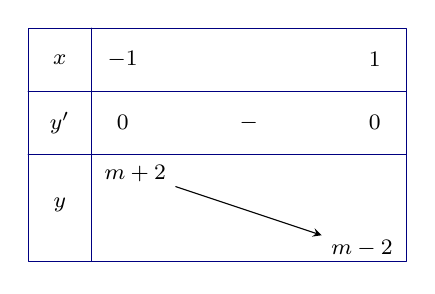
\begin{tikzpicture}[scale=.8,line join=round, line cap=round,font=\footnotesize,>=stealth]
				\def\a{6}
				\def\b{3.7}
				\draw[shift={(-.5,.5)},blue!50!black]
				(0,0) rectangle +(\a,-\b)
				(0,-1)--+(0:\a)
				(0,-2)--+(0:\a)
				(1,0)--+(-90:\b)
				;
				\path
				(0,0) node{$x$}
				(0,-1) node{$y'$}
				(0,-2.3) node{$y$}
				(1,0) node{$-1$}
				(5,0) node{$1$}
				(1,-1) node{$0$}
				(3,-1) node{$-$}
				(5,-1) node{$0$}
				(1.2,-1.8) node (A) {$m+2$}
				(4.8,-3) node (C){$m-2$}
				;
				\draw[->] (A)--(C);
		\end{tikzpicture}}
		\noindent Từ bảng biến thiên của hàm số $y=f(x)$, ta có $\displaystyle\min\limits_{[-1;1]}\left|x^3-3x+m \right|=2$ khi và chỉ khi
		\begin{enumerate}[TH1.]
			\item $\heva{&m+2<0\\&m+2=-2}\Leftrightarrow m=-4$.
			\item $\heva{&m-2>0\\&m-2=2}\Leftrightarrow m=4$.
		\end{enumerate}
		Vậy $S=\{-4,4\}\Rightarrow $ Tổng các phần tử của $S$ bằng $0$.
	}
\end{ex} \dongcham{12}

\Closesolutionfile{ans}


